\documentclass[11pt]{article}
\usepackage[margin=0.9in]{geometry}
\usepackage[T1]{fontenc}
\usepackage{lmodern}
\usepackage{amsmath,amssymb,booktabs}
\usepackage{graphicx}
\usepackage[dvipsnames]{xcolor}
\usepackage{tikz}
\usetikzlibrary{arrows.meta,positioning}
\usepackage{caption}
\usepackage{subcaption}
\graphicspath{{../../outputs/}}
\newcommand{\AP}{\mathrm{AP}}
\newcommand{\PQSTF}{\textsc{PQ-STF}}
\newcommand{\IESTF}{\textsc{IE-STF}}
\title{Experiment Summary: PointPillars, BELT-Fusion, Spatial TrackFormer, and Quantization}
\author{}
\date{}
\begin{document}
\maketitle

\section{PointPillars Late-Fusion Baseline}

We used the published OpenCOOD PointPillars late-fusion checkpoint (\texttt{net\_epoch30.pth}) as the detector baseline. Each CAV runs PointPillars on local LiDAR, predicts 3D boxes $b=(x,y,z,h,w,l,\psi)$ and confidence $s$, transforms source boxes into the ego frame, sends box geometry plus confidence, and ego pools the received detections using late-fusion post-processing/NMS.

\begin{table}[h]
\centering
\caption{Official clean OPV2V test, published PointPillars late-fusion checkpoint.}
\begin{tabular}{lccc}
\toprule
Method & $\AP@0.3$ & $\AP@0.5$ & $\AP@0.7$\\
\midrule
PointPillars naive late fusion & 0.867 & 0.859 & 0.782\\
\bottomrule
\end{tabular}
\end{table}

\paragraph{Important AP convention.} OpenCOOD has an optional \texttt{--global\_sort\_detections} mode. With global sorting, all detections from the full split are ranked jointly before computing the precision--recall curve. Without it, ranking is accumulated in the ordinary evaluation order. These conventions can give substantially different AP, particularly for the SWFormer branch; results must only be compared when the same convention is used.

\paragraph{Conclusion.} PointPillars is the active LiDAR backbone because it is the published, functioning detector checkpoint and gives the strongest clean detector result currently available in this project.

\section{Spatial TrackFormer: Temporal Tracking Adapted to Spatial Association}

\subsection{What original TrackFormer does}

Original TrackFormer performs temporal multi-object tracking. Frame $t-1$ supplies object query states; frame $t$ supplies a new image feature memory. A Transformer decoder propagates the old queries through the new memory, then classifies, regresses, and matches the updated queries. In short, its context is \emph{the same object in adjacent timestamps}.

\subsection{What ``spatial'' means in this project}

We replaced the temporal relation with a same-timestamp cross-agent relation. A source CAV takes the role of the earlier frame and ego takes the role of the current frame. The objective is no longer ``is this object still present at $t$?'' but ``does source proposal $k$ and ego proposal $j$ describe the same physical OPV2V vehicle at this timestamp?''

\begin{figure}[h]
\centering
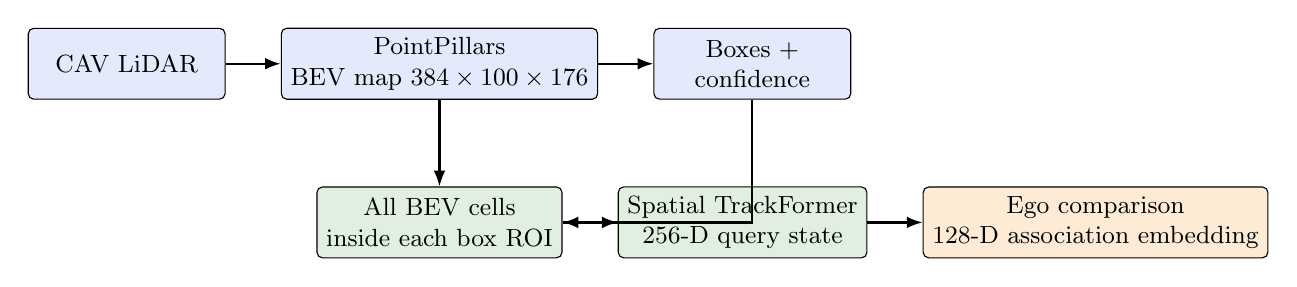
\begin{tikzpicture}[font=\small,box/.style={draw,rounded corners=2pt,align=center,minimum height=9mm,minimum width=25mm,fill=#1!14},arrow/.style={-{Latex[length=2mm]},thick},node distance=7mm]
\node[box=RoyalBlue] (lidar) {CAV LiDAR};
\node[box=RoyalBlue,right=of lidar] (pp) {PointPillars\\BEV map $384\times100\times176$};
\node[box=RoyalBlue,right=of pp] (det) {Boxes +\\confidence};
\node[box=ForestGreen,below=11mm of pp] (roi) {All BEV cells\\inside each box ROI};
\node[box=ForestGreen,right=of roi] (encoder) {Spatial TrackFormer\\256-D query state};
\node[box=BurntOrange,right=of encoder] (ego) {Ego comparison\\128-D association embedding};
\draw[arrow] (lidar)--(pp); \draw[arrow] (pp)--(det); \draw[arrow] (pp.south)--(roi.north); \draw[arrow] (det.south)|-(roi.east); \draw[arrow] (roi)--(encoder); \draw[arrow] (encoder)--(ego);
\end{tikzpicture}
\caption{Spatial TrackFormer interface. The 384-D PointPillars BEV map remains local; only per-object association messages are communicated.}
\end{figure}

For a detected box $k$, its rotated ROI covers $C$ BEV cells. Every cell provides a 384-D PointPillars feature and a 2-D relative position. The box contributes a 9-D geometry/confidence vector. The model projects these three inputs to 256-D and adds them:
\begin{equation}
x_{k,r}=W_FF(r)+\phi_p(p_r)+\phi_g(g_k),\qquad X_k\in\mathbb{R}^{C\times256}.
\end{equation}
The encoder self-attends over the full $C\times256$ matrix; the decoder converts this ROI memory to one 256-D object query state $h_k$. A geometry-conditioned association head produces a normalized 128-D embedding $z_k$.

\subsection{How top-1 cross-agent association is measured}

For each source proposal with a known OPV2V physical object ID, we compare its embedding against all eligible ego proposals in the same timestamp. We select the ego proposal with highest cosine similarity. Top-1 is correct if that ego proposal has the same physical object ID as the source proposal. This measures association identity quality, not final detection AP.

\begin{table}[h]
\centering
\caption{Spatial TrackFormer association results.}
\begin{tabular}{lcc}
\toprule
Evaluation & Top-1 association & Interpretation\\
\midrule
Clean validation & 0.915 & model selection result\\
Clean official test & 0.891 & held-out association result\\
Noisy validation, clean model & 0.907 & association remains robust\\
Noisy official test, clean model & 0.891 & association remains robust\\
\bottomrule
\end{tabular}
\end{table}

\paragraph{Conclusion.} The all-ROI-cell spatial TrackFormer representation successfully distinguishes object identity across CAVs. High top-1 does not automatically imply equally high final AP because AP also depends on matching policy and how matched boxes are fused.

\section{Two Communication Protocols: PQ-STF versus IE-STF}

Both protocols use the same \emph{local} object encoder.  For every detected box, a CAV extracts every BEV cell covered by its rotated ROI, projects the PointPillars cell feature, cell position, and box geometry/confidence to 256 dimensions, and processes the resulting $C\times256$ ROI-token matrix with the Transformer encoder.  The difference is strictly what is transmitted and what ego does with it.

\begin{figure}[h]
\centering
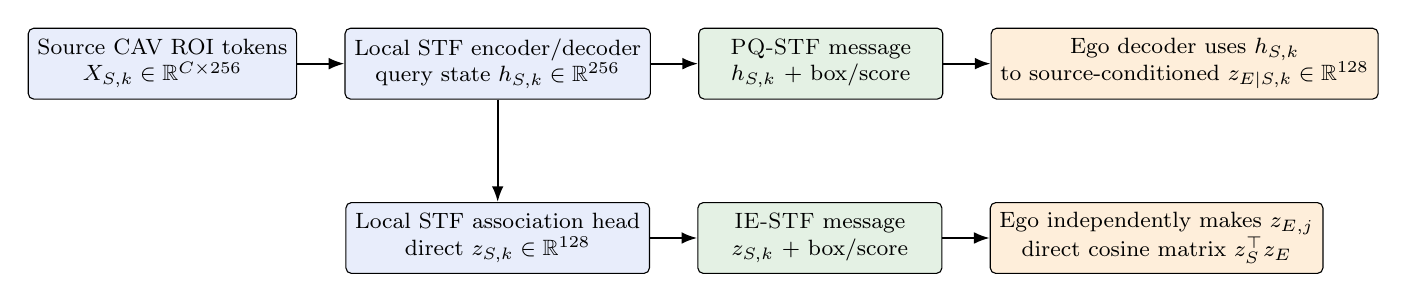
\begin{tikzpicture}[font=\footnotesize,box/.style={draw,rounded corners=2pt,align=center,minimum height=9mm,minimum width=31mm,fill=#1!12},arrow/.style={-{Latex[length=2mm]},thick},node distance=6mm]
\node[box=RoyalBlue] (srcroi) {Source CAV ROI tokens\\$X_{S,k}\in\mathbb{R}^{C\times256}$};
\node[box=RoyalBlue,right=of srcroi] (srcenc) {Local STF encoder/decoder\\query state $h_{S,k}\in\mathbb{R}^{256}$};
\node[box=ForestGreen,right=of srcenc] (pqmsg) {\PQSTF\ message\\$h_{S,k}$ + box/score};
\node[box=BurntOrange,right=of pqmsg] (pqego) {Ego decoder uses $h_{S,k}$\\to source-conditioned $z_{E\mid S,k}\in\mathbb{R}^{128}$};
\draw[arrow] (srcroi)--(srcenc); \draw[arrow] (srcenc)--(pqmsg); \draw[arrow] (pqmsg)--(pqego);
\node[box=RoyalBlue,below=13mm of srcenc] (ieenc) {Local STF association head\\direct $z_{S,k}\in\mathbb{R}^{128}$};
\node[box=ForestGreen,right=of ieenc] (iemsg) {\IESTF\ message\\$z_{S,k}$ + box/score};
\node[box=BurntOrange,right=of iemsg] (iego) {Ego independently makes $z_{E,j}$\\direct cosine matrix $z_S^\top z_E$};
\draw[arrow] (srcenc.south)--(ieenc.north); \draw[arrow] (ieenc)--(iemsg); \draw[arrow] (iemsg)--(iego);
\end{tikzpicture}
\caption{The essential protocol difference. PQ-STF sends a 256-D query state that ego consumes inside its decoder; IE-STF sends a directly comparable 128-D embedding.  In both cases, box geometry and confidence remain necessary for final box fusion.}
\end{figure}

\subsection{PQ-STF: propagated-query Spatial TrackFormer}

For a source object $k$, the CAV sends the decoder query state $h_{S,k}\in\mathbb{R}^{256}$, not merely a finished identity vector.  Ego encodes its own proposal ROIs, inserts $h_{S,k}$ as a propagated query in its decoder, and obtains a source-conditioned ego representation $z_{E\mid S,k}\in\mathbb{R}^{128}$.  ``Source-conditioned'' means the ego-side representation is recomputed after attention to that particular received source state; a different source state can yield a different ego representation.  Source and ego association embeddings are then compared with cosine similarity, subject to the physical plausibility condition.

This is the more expressive protocol: ego can use source appearance/context while interpreting its own ROI.  Its raw association-state payload is $256\times32=8192$ bits $=1024$ B per selected source object, before box/score and networking metadata.

\subsection{IE-STF: independent-embedding Spatial TrackFormer}

IE-STF means \emph{independent-embedding Spatial TrackFormer}.  Each CAV uses its local ROI memory and association head to produce a final normalized $z_{S,k}\in\mathbb{R}^{128}$; ego independently produces $z_{E,j}\in\mathbb{R}^{128}$ for its own boxes.  Ego forms the $N_S\times N_E$ cosine-similarity matrix directly.  No received source state enters ego's decoder, so the transmitted 128-D vectors are deployment-friendly and immediately comparable.

\begin{table}[h]
\centering
\caption{Protocol comparison on the official clean OPV2V test. Payloads are association-state payloads only.}
\begin{tabular}{p{28mm}p{34mm}p{34mm}}
\toprule
& \PQSTF & \IESTF\\
\midrule
Transmitted learned representation & 256-D decoder query state $h_S$ & 128-D direct embedding $z_S$\\
What ego does & Reuses $h_S$ inside ego decoder, then compares conditioned embeddings & Independently embeds ego boxes and compares directly\\
Raw float32 state payload & 1024 B/object & 512 B/object\\
Clean top-1 association & 0.891 & 0.881\\
Clean BELT AP@0.7 & 0.765 & 0.744\\
\bottomrule
\end{tabular}
\end{table}

\paragraph{Conclusion.} IE-STF is cheaper before quantization, but current PQ-STF is stronger both in held-out association and end-to-end AP.  The rest of the quantization study therefore focuses on PQ-STF.

\section{Noise Sensitivity and Annealing}

The geometry-noise study uses Gaussian position error and heading error. Position error shifts the source box centre; heading error rotates the source box. We tested position-only, heading-only, and paired position+heading perturbations during association studies. For end-to-end cooperative detection, the main figure uses paired values $(0\text{ m},0^\circ)$, $(1\text{ m},5^\circ)$, $(2\text{ m},10^\circ)$, $(4\text{ m},20^\circ)$, and $(10\text{ m},30^\circ)$.

The annealed model was trained through progressively stronger geometry-only noise stages. Its purpose is to trade some clean specialization for better resistance at larger localization error. It is not expected to be best at every noise point.

\begin{figure}[h]
\centering
\includegraphics[width=0.93\linewidth]{geometry_only_noise_sweep/extreme_geometry_clean_vs_curriculum.png}
\caption{Cross-agent top-1 association sensitivity under geometry-only localization noise. Color identifies the perturbation type: position only, heading only, or both. Solid lines are the clean-trained PQ-STF encoder; dashed lines are the annealed encoder. At $\alpha=1$, the applied standard deviations are 1 m and/or $5^\circ$; subsequent points use $(2\text{ m},10^\circ)$, $(4\text{ m},20^\circ)$, and $(10\text{ m},30^\circ)$. Higher is better.}
\label{fig:association-sensitivity}
\end{figure}

\paragraph{How to read Fig.~\ref{fig:association-sensitivity}.} This figure isolates the encoder's \emph{identity matching}: for each source proposal, does its highest-cosine ego proposal have the same physical OPV2V object ID?  It is not AP and does not contain box fusion.  The clean encoder begins around 0.89 top-1 at zero noise and loses identity discrimination rapidly at stronger perturbations.  Annealing starts lower on clean data (dashed lines at $\alpha=0$) but is substantially less sensitive as position/heading error grows.  Position-only, heading-only, and combined curves show which perturbation type creates the loss; combined noise is the operational stress case.

\begin{figure}[h]
\centering
\includegraphics[width=0.92\linewidth]{belt_geometry_noise_sweep/ap70_geometry_noise_comparison.png}
\caption{End-to-end vehicle AP@0.7 under combined position/heading localization noise. This is the AP study, not the association top-1 study. Every TrackFormer curve is \emph{PQ-STF with BELT}: source CAVs transmit propagated 256-D query states, ego conditions its decoder on them, and BELT performs final uncertainty-aware box fusion. ``Annealed PQ-STF + codebook + BELT'' uses an 8-B query-state code, a $1024/8=128\times$ reduction of the raw 1024-B association state; geometry/score and protocol overhead are excluded from that ratio.}
\end{figure}

\begin{table}[h]
\centering
\caption{AP@0.7 values used in the combined localization-noise figure. All PQ-STF rows use propagated-query association and BELT box fusion; they are not IE-STF or simple-fusion results.}
\begin{tabular}{lccccc}
\toprule
Method & $0/0^\circ$ & $1/5^\circ$ & $2/10^\circ$ & $4/20^\circ$ & $10/30^\circ$\\
\midrule
Naive PointPillars & .782 & .250 & .268 & .400 & .568\\
Clean-trained PQ-STF + BELT & .711 & .456 & .352 & .378 & .510\\
Annealed PQ-STF + BELT & .683 & .425 & .343 & .388 & .533\\
Annealed PQ-STF + 8-B codebook + BELT & .677 & .419 & .339 & .388 & .527\\
\bottomrule
\end{tabular}
\end{table}

\paragraph{Why AP rises again after extreme noise.} All cooperative association paths use a physical distance condition of at most 5 m. Once noisy source boxes move farther than this, they are not included in a multi-agent fusion group. The number of fused boxes falls and more detections remain local/singleton boxes. Therefore the $10$-m/$30^\circ$ point is not evidence that extreme localization noise improves perception; it shows that the system is performing less cooperative box fusion.

\paragraph{Conclusion.} Annealing changes the robustness trade-off, but the AP curve must always be interpreted with the number of accepted groups and final boxes. Top-1 association and final AP answer different questions.

\section{BELT-Fusion: Geometry Association and Uncertainty-Aware Box Fusion}

All main end-to-end TrackFormer experiments initially used BELT because it supplies both a grouping rule and a robust box-fusion rule.

\subsection{BELT association}

Every source box is transformed into ego coordinates. For a current group representative centre $\mu_G$ and a candidate centre $c_j$, geometry association uses a one-to-one Hungarian assignment based on centre distance, accepting an association only when
\begin{equation}
d(G,j)=\lVert\mu_G-c_j\rVert_2\leq5\ \mathrm{m}.
\end{equation}
TrackFormer replaces the assignment preference with cosine similarity of learned association embeddings, while retaining the 5-m physical plausibility condition.  With source objects $k$ and ego objects $j$, the association is a one-to-one Hungarian assignment over the valid pairs,
\begin{equation}
M^*=\arg\max_M\sum_{(k,j)\in M}\cos(z_{S,k},z_{E,j})
\quad\text{s.t.}\quad\lVert c_{S,k}-c_{E,j}\rVert_2\leq5\ \mathrm{m},\quad \cos(z_{S,k},z_{E,j})\geq0.90.
\end{equation}
The $5$-m condition rejects geometrically implausible pairs; the 0.90 cosine gate rejects semantically dissimilar pairs.

\subsection{What happens to detections without an overlap}

Association does \emph{not} discard a detection merely because no other CAV observed the same vehicle.  Ego detections begin as singleton groups.  A matched source proposal is appended to its ego group and the group is fused.  An ego-only proposal remains a singleton and its own box is retained.  Likewise, a source-only proposal that has no valid ego match becomes a singleton source group; after transformation to ego coordinates, it is emitted as an additional cooperative detection rather than being dropped.  Standard final post-processing/NMS can still suppress duplicate output boxes.

The present PQ-STF association is deliberately \emph{ego-centric}: each source CAV is matched independently against ego proposals.  Consequently, if ego misses a vehicle but two non-ego CAVs both detect it, those two source proposals are not currently joined and fused with each other by PQ-STF; they remain separate singleton candidates, subject only to final NMS.  A future all-agent association graph would add source--source edges, cluster every mutually matching proposal, and allow BELT to fuse a source-only multi-CAV group.

\subsection{BELT box fusion}

The uncertainty model predicts a covariance $\Sigma_i$ for each box. Once a group is associated, BELT fuses box means by precision weighting:
\begin{equation}
\Sigma_f^{-1}=\sum_i\Sigma_i^{-1},\qquad \mu_f=\Sigma_f\sum_i\Sigma_i^{-1}\mu_i.
\end{equation}
Thus a high-uncertainty box has low precision and cannot move the fused result strongly. Classification evidence is represented by Dirichlet parameters $\alpha_c=e_c+1$, with uncertainty decreasing as total evidence $S=\sum_c\alpha_c$ increases.

\begin{table}[h]
\centering
\caption{Canonical noisy OPV2V test: $0.2$-m position noise, $0.2^\circ$ heading noise, 100-ms delay.}
\begin{tabular}{lccc}
\toprule
Method & $\AP@0.3$ & $\AP@0.5$ & $\AP@0.7$\\
\midrule
Naive late fusion & .860 & .712 & .294\\
BELT geometry association + BELT fusion & .851 & .752 & .415\\
\PQSTF association + BELT fusion & .846 & .743 & .423\\
\bottomrule
\end{tabular}
\end{table}

\paragraph{Conclusion.} The large noisy gain ($.294\rightarrow.415$) comes from BELT uncertainty-aware fusion. TrackFormer changes cross-agent association and provides a smaller further strict-AP gain ($.415\rightarrow.423$).

\section{Separating PQ-STF from BELT}

\PQSTF means \emph{propagated-query Spatial TrackFormer}. A source CAV sends the 256-D query state $h_{S,k}$ for each selected source object, together with normal box geometry and confidence. Ego runs its own ROI encoder, injects the received query states into the decoder, obtains source-conditioned ego embeddings, computes cosine similarity, and forms one-to-one source--ego associations.

To isolate association from BELT, we created a PQ-STF-only branch: the same propagated-query association is used, but associated boxes are combined by detector-score-weighted averaging instead of uncertainty/covariance fusion. Clean results are below.

\paragraph{Scope clarification.} This ablation contains clean PQ-STF at raw, 4-B, 2-B, and 1-B query-state rates, plus the raw-state annealed sweep below.  Fig.~4 and Table~4 remain strictly \emph{annealed PQ-STF + BELT} results, never annealed simple-fusion results.

The annealed PQ-STF-only/raw-state sweep has now been completed at all four non-zero combined-noise points.  It uses the same propagated-query association and fixed 5-m/0.90 gates as the BELT study, but replaces BELT's covariance/evidential fusion with detector-score-weighted averaging.  There is intentionally no ``clean'' point in this table: the existing clean PQ-STF-only experiment used the clean-trained checkpoint, not the annealed checkpoint.

\begin{table}[h]
\centering
\caption{Annealed PQ-STF-only (raw 1024-B query state): no BELT box fusion. The decreasing group count shows that extreme noise leaves almost all detections unmatched/singleton.}
\begin{tabular}{lrrrr}
\toprule
Combined noise & $1$ m/$5^\circ$ & $2$ m/$10^\circ$ & $4$ m/$20^\circ$ & $10$ m/$30^\circ$\\
\midrule
$\AP@0.7$ & .2208 & .2538 & .4009 & .5664\\
Multi-agent groups/frame & 1.118 & .547 & .259 & .034\\
Final boxes/frame & 32.92 & 33.60 & 33.96 & 34.19\\
\bottomrule
\end{tabular}
\end{table}

\paragraph{Interpretation.} At 1--2 m, removing BELT substantially reduces strict AP because score-weighted averaging cannot account for unreliable box geometry.  At 10 m/$30^\circ$, almost no pairs pass the 5-m association condition, so the system mostly emits local/singleton detections; the apparent AP increase is therefore reduced cooperation, not successful fusion under extreme error.

\begin{table}[h]
\centering
\caption{PQ-STF-only clean test: fixed cosine gate 0.90, score-weighted box average, no BELT fusion.}
\begin{tabular}{lccc}
\toprule
Query-state payload & $\AP@0.7$ & Groups/frame & Boxes/frame\\
\midrule
Raw 1024 B & .7364 & 7.08 & 23.66\\
Fixed 4 B & .7361 & 6.36 & 25.15\\
Fixed 2 B & .7394 & 5.70 & 26.42\\
Fixed 1 B & .7457 & 4.30 & 28.59\\
\bottomrule
\end{tabular}
\end{table}

\paragraph{Conclusion.} BELT is important for absolute AP: raw PQ-STF-only gives .7364 AP@0.7, whereas raw PQ-STF+BELT gives .7655. Strong compression reduces accepted groups; it can avoid harmful incorrect averages, which explains why a lower-rate message can appear slightly better in this particular discrete fusion setup. It does not mean compressed embeddings are intrinsically better.

\section{Codebook Quantization and Adaptive Communication}

The compressed quantity is the \PQSTF 256-D float32 query state. Raw cost is $256\times32=8192$ bits $=1024$ bytes per selected source object. This number excludes transmitted box geometry, confidence, uncertainty/rate tags, headers, and network overhead.

\begin{table}[h]
\centering
\caption{BELT+PQ-STF clean test: fixed residual query-state quantization.}
\begin{tabular}{lrrrr}
\toprule
State payload & Compression & Bytes/frame & $\AP@0.7$ & Groups/frame\\
\midrule
Raw 1024 B & $1\times$ & 21935.8 & .76546 & 7.08\\
16 B & $64\times$ & 342.7 & .76551 & 6.79\\
8 B & $128\times$ & 171.4 & .76540 & 6.35\\
4 B & $256\times$ & 85.7 & .76475 & 5.16\\
\bottomrule
\end{tabular}
\end{table}

\begin{figure}[h]
\centering
\includegraphics[width=0.84\linewidth]{pq_stf_compression_tradeoff/clean_ap70_vs_compression.png}
\caption{How to read the fixed-rate compression trade-off. Each categorical x-axis label gives the query-state payload per selected source object and its compression factor relative to raw 1024 B. The y-axis is clean end-to-end AP@0.7 in percent; it is intentionally zoomed around 76.5\% to reveal the small differences. The plot shows that 4--16 B retains essentially the same measured AP as raw state, while transmitting 64--256$\times$ fewer association-state bytes.}
\end{figure}

\subsection{What the uncertainty figures measure}

The BELT uncertainty network is evaluated at the \emph{source CAV}, for every transmitted source proposal.  It predicts class uncertainty, position standard deviation, and heading standard deviation.  For analysis, a proposal is called \emph{matched} if its detector box has ground-truth IoU at least 0.5, otherwise \emph{unmatched}.  This label is used only offline to inspect calibration; it is not sent at deployment.

\begin{figure}[h]
\centering
\includegraphics[width=0.96\linewidth]{belt_uncertainty_clean_test_distribution/source_proposal_uncertainty_pdf.png}
\caption{Probability density functions for source-proposal uncertainty on the official clean test set. Blue curves are ground-truth matched detector proposals; orange curves are unmatched proposals. The orange distributions shift toward higher uncertainty for classification, position, and heading, which provides a source-local signal for allocating more message bits to riskier detections.}
\label{fig:uncertainty-pdf}
\end{figure}

\subsection{How adaptive rate is selected}

The source combines its uncertainty predictions into a scalar score and ranks only its own selected proposals in that frame.  Let $r\in[0,1]$ be this within-source uncertainty rank.  Thresholds are calibrated \emph{once} on held-out validation scenarios to meet a desired average communication budget, by allocating longer residual prefixes preferentially to proposals that look like unmatched/risky detections.  For the 1/2/4-B policy with a target of approximately 2 B per source object, calibration selected $t_1=0.61$ and $t_2=0.64$:
\begin{equation}
q(r)=\begin{cases}
1\ \mathrm{B}, & r\leq0.61,\\
2\ \mathrm{B}, & 0.61<r\leq0.64,\\
4\ \mathrm{B}, & r>0.64.
\end{cases}
\end{equation}
Thus the high-uncertainty tail obtains more residual stages.  The CAV transmits the resulting code indices plus a small rate tag; ego uses the tag to decode the received prefix into an approximate 256-D query state.  No ego-to-source uncertainty feedback is required, and this threshold selection is a validation-calibrated policy, not end-to-end differentiable training.

\begin{figure}[h]
\centering
\includegraphics[width=0.96\linewidth]{belt_uncertainty_rate_calibration_1_2_4b_validation/adaptive_rate_calibration.png}
\caption{Validation-calibrated adaptive coding policy. Left: matched and unmatched source proposals separate by within-source uncertainty rank; dashed lines are $t_1=0.61$ and $t_2=0.64$. Right: the learned allocation gives most low-uncertainty proposals 1 B and gives high-uncertainty, more often unmatched proposals 4 B. This explains the adaptive mechanism rather than merely reporting its final mean rate.}
\label{fig:adaptive-rate}
\end{figure}

For adaptive coding, the source CAV ranks its own proposals by class uncertainty, predicted position standard deviation, and predicted heading standard deviation. Two validation-calibrated thresholds choose a 1-B, 2-B, or 4-B residual prefix. Ego receives the code indices and a rate tag, then reconstructs the same 256-D state approximation. This is source-local: ego does not send uncertainty feedback to the CAV.

\begin{table}[h]
\centering
\caption{Adaptive 1/2/4-B residual coding, official clean test.}
\begin{tabular}{lcccc}
\toprule
Policy & Mean state payload & State reduction & $\AP@0.7$ & Meaning\\
\midrule
Raw PQ-STF state & 1024 B/object & --- & .76546 & full float32 $h_S$\\
Adaptive residual state & 2.04 B/object & 99.80\% & .76708 & 1/2/4-B selected by Fig.~\ref{fig:adaptive-rate}\\
\bottomrule
\end{tabular}
\end{table}

\paragraph{Conclusion.} The correct statement is ``99.80\% association-state bandwidth reduction with no material observed AP loss.'' The $0.16$ percentage-point AP difference is too small and affected by changed grouping decisions; it is not evidence that quantization improves the learned representation.

\clearpage

\section{Independent-Embedding Protocol and SWFormer Branch}

\IESTF (independent-embedding Spatial TrackFormer) was trained from scratch so every CAV sends a direct 128-D embedding rather than a propagated 256-D query state. It achieved .881 clean-test top-1 association but .744 AP@0.7 end-to-end with BELT, below PQ-STF's .765. It remains a valid lower-bandwidth protocol branch but is not the current preferred design.

We also integrated OpenCOOD-SWFormer as a separate LiDAR backbone experiment. SWFormer uses sparse voxel tokens and shifted-window attention instead of PointPillars' dense 2D CNN BEV backbone. The current single-sweep SWFormer runs reached approximately .69/.69/.68 AP at IoU .3/.5/.7 under globally sorted evaluation, below the PointPillars .867/.859/.782 baseline. PointPillars therefore remains the backbone used for all TrackFormer and communication results.

\section{Current Conclusions}

\begin{enumerate}
\item Published PointPillars late fusion is the strongest current clean detector baseline.
\item BELT uncertainty-aware fusion is the main mechanism recovering strict AP under noisy localization.
\item Spatial TrackFormer successfully learns cross-agent vehicle identity from all PointPillars ROI cells; PQ-STF is currently stronger than IE-STF end-to-end.
\item Annealed training improves the robustness trade-off but must be interpreted jointly with the number of accepted fusion groups.
\item Query-state quantization is highly effective: 4-B fixed coding and 2.04-B adaptive coding preserve clean AP to within a negligible observed difference.
\item The next controlled branch is the completed noisy PQ-STF-only compression curve at all paired position/heading noise points, followed by fixed-rate versus adaptive-rate comparison at matched payload under noise.
\end{enumerate}

\end{document}
